\index{wing nuts}
\index{filament spool}
\index{spool}
\glossary{Spool}{Plastic Filament coiled and stored on a plastic reel. Preferred due to improved feeding and better mounting options.}
\glossary{Filament}{Plastic material in "string" like form, as is fed to the printer.}
\glossary{ABS}{Acrylonitrile Butadiene Styrene thermoplastic. Usually extrudes at 230C.}
\glossary{PLA}{Polylactic Acid is a corn-based biodegradable polymer. Usually extrudes at 185C.}
\glossary{HDPE}{High Density Polyethylene.}
\glossary{Polycarbonate}{A strong and impact resistant thermoplastic. Usually extrudes at ~300C.}
\glossary{HIPS}{High Impact Polystyrene.}
\glossary{Laywoo-D3}{Wooden filament similar to PLA. Contains 40 percent recycled wood. Usually prints at ~180C- 210C. Color can be changed by varying the extrusion temperature.}
\begin{figure}[hbt]
\centering
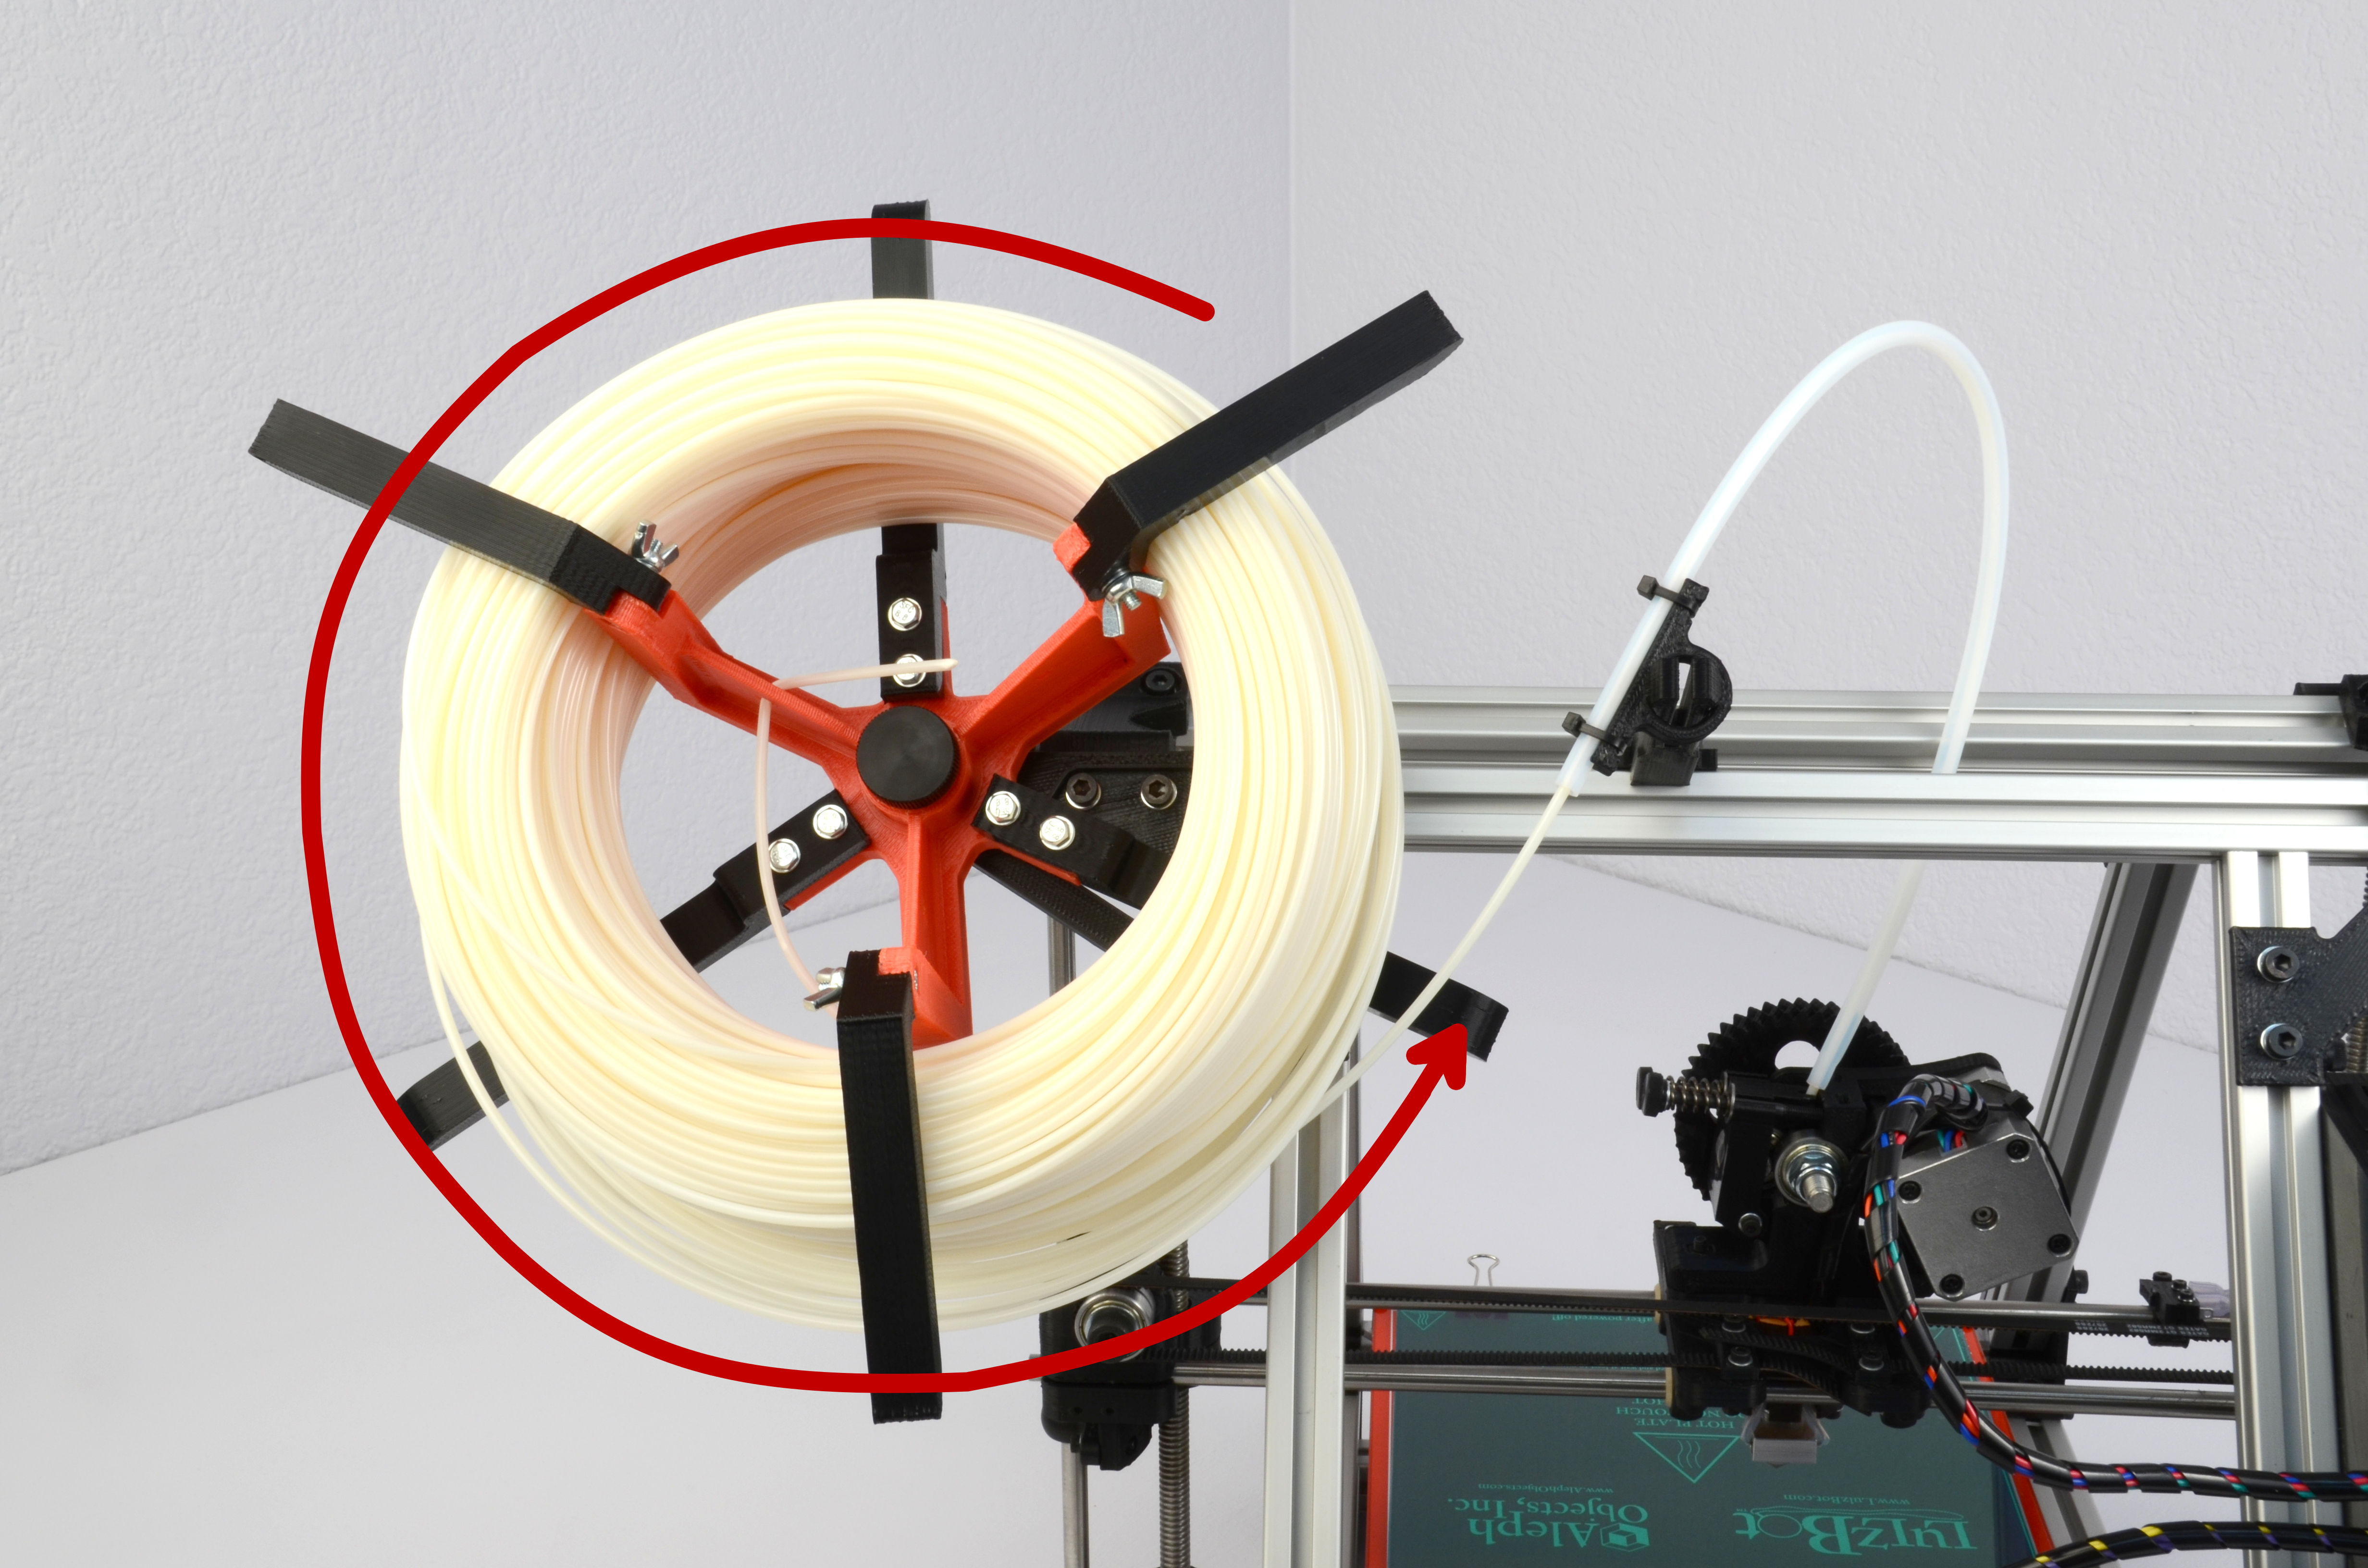
\includegraphics[keepaspectratio=true,angle=0,height=0.4\textheight,width=1.0\textwidth]{filament_spool_dir.jpg}
\caption{Filament spool direction}
\label{fig:filament_spool_dir}
\end{figure}
\begin{enumerate}
\item Loosen the three wing nuts on the upper arms of the filament spool.

\item Turn the upper arms 90 degrees upwards away from the printer.

%\glossary{Coil}{Raw filament.}

\item Remove the 5lb coil of filament from the plastic packaging, leaving the twist ties on.

\item Slide the coil over the spool upper arms. Make sure the filament coil direction is counter clock wise (from the rear of the printer) when placing the coil on to the spool
(Fig. \ref{fig:filament_spool_dir}, page \pageref{fig:filament_spool_dir}).

\item Lower the three upper arms and re-tighten the wing nuts.

\item The twist ties can now be removed. Keep the twist ties for future use if you ever need to remove the filament to change to a different filament.

\index{feed tube}
\item Feed the end of the filament through the filament feed tube.

\item If it is loose, slide the opposite end of the filament through one of the holes in hub of the filament spool. This will keep the filament from unwinding from the spool.

\end{enumerate}
